\documentclass[9pt]{article}
\usepackage{amssymb,amsmath}
\usepackage{ifxetex,ifluatex}
\usepackage{fixltx2e} % provides \textsubscript
\ifnum 0\ifxetex 1\fi\ifluatex 1\fi=0 % if pdftex
  \usepackage[T1]{fontenc}
  \usepackage[utf8]{inputenc}
\else % if luatex or xelatex
  \ifxetex
    \usepackage{mathspec}
    \usepackage{xltxtra,xunicode}
  \else
    \usepackage{fontspec}
  \fi
  \defaultfontfeatures{Mapping=tex-text,Scale=MatchLowercase}
  \newcommand{\euro}{€}
\fi
% use upquote if available, for straight quotes in verbatim environments
\IfFileExists{upquote.sty}{\usepackage{upquote}}{}
% use microtype if available
\IfFileExists{microtype.sty}{%
\usepackage{microtype}
\UseMicrotypeSet[protrusion]{basicmath} % disable protrusion for tt fonts
}{}
\usepackage{graphicx}
\makeatletter
\def\maxwidth{\ifdim\Gin@nat@width>\linewidth\linewidth\else\Gin@nat@width\fi}
\def\maxheight{\ifdim\Gin@nat@height>\textheight\textheight\else\Gin@nat@height\fi}
\makeatother
% Scale images if necessary, so that they will not overflow the page
% margins by default, and it is still possible to overwrite the defaults
% using explicit options in \includegraphics[width, height, ...]{}
\setkeys{Gin}{width=\maxwidth,height=\maxheight,keepaspectratio}
\ifxetex
  \usepackage[setpagesize=false, % page size defined by xetex
              unicode=false, % unicode breaks when used with xetex
              xetex]{hyperref}
\else
  \usepackage[unicode=true]{hyperref}
\fi
\hypersetup{breaklinks=true,
            bookmarks=true,
            pdfauthor={},
            pdftitle={3 Ethical Theories},
            colorlinks=true,
            citecolor=blue,
            urlcolor=blue,
            linkcolor=magenta,
            pdfborder={0 0 0}}
\urlstyle{same}  % don't use monospace font for urls
\setlength{\parindent}{0pt}
\setlength{\parskip}{6pt plus 2pt minus 1pt}
\setlength{\emergencystretch}{3em}  % prevent overfull lines
\setcounter{secnumdepth}{0}

\title{3 Ethical Theories}
\author{Scott O'Connor}

\begin{document}
\maketitle


\subsection{Introduction}\label{introduction}

Study last week's handout. Recall that there are 3 ethical theories. In
this handout, I will provide some further details about these theories.
The textbook contains a fuller explanation as well as objections.

\subsection{Consequentialism}\label{consequentialism}

\begin{figure}[htbp]
\centering
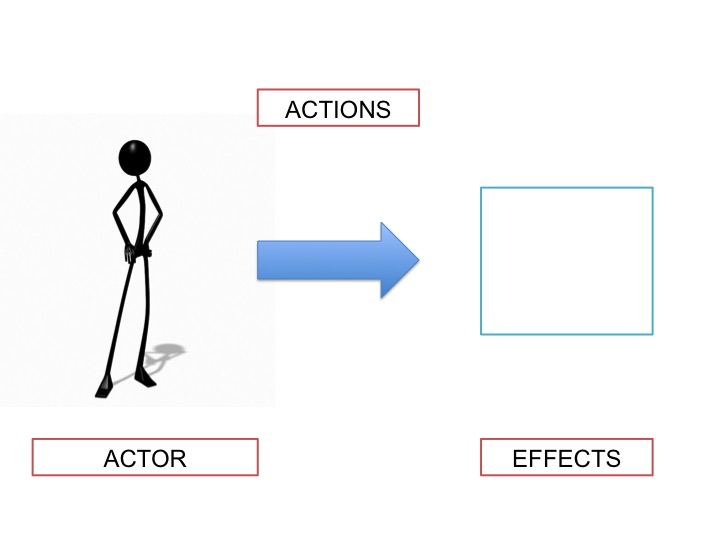
\includegraphics{Slide1.jpg}
\end{figure}

Consequentialists claim that morality depends completely on the effects
of our actions. They say that the actor side of the diagram is
irrelevant as is the intrinsic nature of their acts.

There are different versions of Consequentialism. They differ,
primarily, in what effects they construe as relevant for morality.
\textbf{Egoism} says that right actions are those that further one's own
best interests. Egoists say that the effects your actions have on others
is irrelevant to the morality of your actions. All that is relevant is
the effects your actions have on you. For further discussion of Egoism,
see the textbook.

In this handout, I will discuss a second version of Consequentialism.
\textbf{Utilitarianism} agrees that the effects of an action determines
its morality. Unlike the egoist, the utilitarian claims that the effects
actions have on everyone (including yourself) is what determines their
morality. On this view, your action may harm your self interest, but
will still be right if the positive effects of the action on others
outweighs the harms to yourself. Utilitarians accept the following
principle:

\begin{description}
\itemsep1pt\parskip0pt\parsep0pt
\item[The Principle of Utility:]
Rights actions are those that result in greater overall well-being (or
utility) for the people involved than any other possible action.
\end{description}

Consider torture. The police learn that a person S has planted a bomb
somewhere in the city. They arrest S who remains silent after intense
questioning. A police officer asks herself, `would it be morally
permissible for me to force an answer using violence, using torture?'
The Consequentialist denies that there are is an absolute moral
prohibition against torture. Whether it is moral depends entirely on the
effects the action will have on the people involved.

What effects should we attend to? Utilitarians disagree on this point.
For our purposes, we can focus on Jeremy Bentham's rather simple view
that the only effects that matter are the pleasures and pains caused by
the action on the people involved. On this view, one should maximize
pleasure and minimize pains regardless of the distribution of those
pleasures and pains. Here we have to consider two scenarios:

\begin{description}
\itemsep1pt\parskip0pt\parsep0pt
\item[Scenario 1:]
The police officer tortures the prisoner. The prisoner experiences much
pain. The officer suffers mental torment. They bomb is found. The
officers feel relief at preventing a tragedy. Nobody suffers the pain of
being injured, maimed by an exposition. Nobody suffers the pain from
dying in an explosion. Nobody suffers the pain of losing a loved one in
an explosion.
\item[Scenario 2:]
The police officer does not torture the prisoner. The prisoner suffers
no physical pain. The officer suffers no mental anguish from torturing
her prisoner. Several people suffer incredible pain from being injured
in the explosion. Many suffer great pain as they die from the explosion.
Many suffer great pain from losing a loved one.
\end{description}

The officer can torture or not. According to Utilitarianism, she should
decide by comparing the prospective pleasures and pains involved in both
scenarios. As presented, scenario 2 involves a far greater ratio of pain
to pleasure than scenario 1. Suppose that we quantify pains and
pleasures. Scenario 1 might result in 20 units of pain and 20 units of
pleasure, which is a ratio of pain to pleasure of 1:1. Scenario 2 might
result in 2000 units of pain and 10 of pleasure, which is a ratio of
pain to pleasure of 200:1. Clearly the first scenario has a better ratio
of pain to pleasure, so, according to the consequentialist, torture is
the morally required thing to do in this circumstance.

\subsection{Rule vs.~Act
Utilitarianism}\label{rule-vs.act-utilitarianism}

Utilitarianism may seem to legitimize such terrible evils that it is
unworthy of our attention. If the choice is between a huge amount of
pleasure for a small group of people or a very small amount of pleasure
for a huge number of people, we should advance the interest of the
minority. Among other things, this legitimizes slavery if the benefits
to the slave owners far outweigh the pain suffered by the slaves. A
terrible result! Utilitarianism, though, is a much more sophisticated
theory than it first appears. There are two very distinct versions of
it:

\begin{description}
\item[Act-utilitarianism:] The rightness of actions depends solely on the
overall well-being produced by individual actions.

\item[Rule-utilitarianism:] A right action is one that conforms to a rule
that, if followed consistently, would create for everyone involved the
most beneficial balance of well-being over suffering.
\end{description}

Act Utilitarianism has the unpleasant results I just mentioned. It says
that the rightness and wrongness of an \emph{individual action} depends
solely on the overall well-being produced by that \emph{individual act}.
Torture in a particular situation is moral because that individual act
of torture produces a greater balance of well-being over suffering than
any alternative action. In a different circumstance, an individual act
of torture is immoral because that individual act produces a worse
balance of well-being over suffering that some alternative. Act
utilitarianism, then, says that an individual act should be isolated
from similar acts and evaluated merely on the basis of that individual
act's effects.

Rule Utilitarianism, on the other hand, says that an individual act
cannot be isolated from similar acts. It claims that the rightness and
wrongness of an act depends on the effects that would be produced by
everyone doing similar acts, i.e., by following a rule that sanctioned
or prohibited that act.

Note that adhering to certain rules to maximize well-being for everyone
involved may require us to perform particular acts that have bad effects
in a particular situation. Consider our torture case once again.

\begin{description}
\itemsep1pt\parskip0pt\parsep0pt
\item[Scenario 1]
The police officer tortures the prisoner. Here the officer is acting as
if it is generally permissible for the police to torture prisoners. What
would the effects of this permission being granted to the police force?
On the one hand, they may stop some crimes using that torture. Perhaps
they will catch a guilty party or two. But this will be far out shadowed
by the turmoil that would ensue. Riots would follow. Few, if any, would
report a crime or cooperate with the police.
\item[Scenario 2]
The police officer does not torture the prisoner. Here the officer is
acting on the assumption that it is never permissible for the police to
torture a prisoner. Here the prisoner suffers no physical pain. The
officer suffers no mental anguish from torturing her prisoner. There is
no civil strife from a corrupt police force which has not lost the trust
of the public. Nevertheless, several people suffer incredible pain from
being injured in the explosion. Many suffer great pain as they die from
the explosion. Many suffer great pain from losing a loved one.
\end{description}

Here we must assess the effects of both rules being implemented and
followed. In Scenario 1, the negative effects may involve a breakdown in
civil society. In Scenario 2, civil society is preserved but the several
acts of terrorism may not be prevented. Nevertheless, the negative
effects in Scenario 1 likely outweigh those in Scenario 2. Thus the Rule
Utilitarian will judge it immoral to torture even though, on occasion,
it might help us avoid some specific negative result.

For more on Utilitarianism, watch the following series of
\href{https://www.youtube.com/watch?v=uvmz5E75ZIA\&list=PLtKNX4SfKpzWiiUdXS9MKf8bgUfQSOlas}{clips.}

\subsection{Deontology}\label{deontology}

\begin{figure}[htbp]
\centering
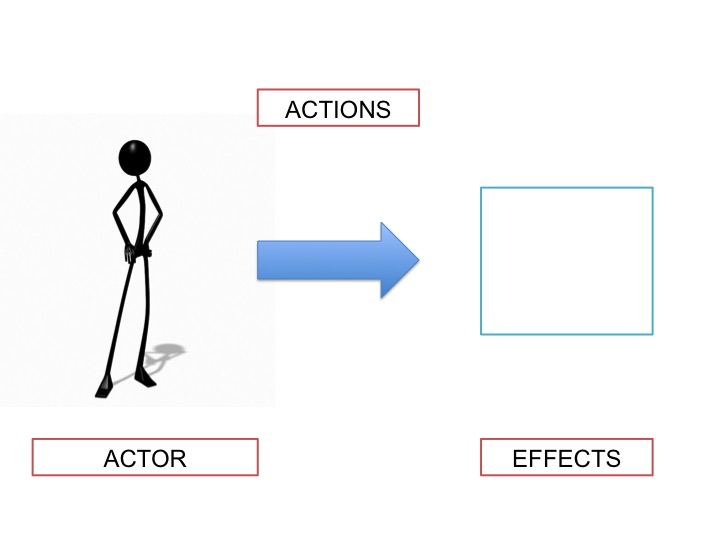
\includegraphics{Slide1.jpg}
\end{figure}

Recall again our diagram. The consequentialist, we have seen, claims
that the effects, and only the effects, are relevant in determining the
morality of our actions. They deny that any facts about the person are
relevant. On the one hand, Deontologist agree that the morality of our
actions has nothing to with the intentions, beliefs, conscience of the
actor. But they also deny that effects have anything to do with the
morality of our actions. They protest that consequentialism ignores a
core feature of morality; we have a duty to do the right thing and a
responsibility to avoid the wrong thing regardless of the consequences.
Actions, on this view, are right or wrong independently of their
effects, production of happiness, people's aims, or their desires and
feelings.

To introduce you to this view, distinguish between two types of value,
inherent vs.~relational value. Relational value is value something has
only in virtue of its relationship to something else that is valuable.
Money has only relational value. It is valuable only in relation to what
you can buy with it. If the human race were to go extinct, but our money
remain, that money would not be something valuable. Health, on the other
hand, is valuable in and of itself. Of course, being healthy helps us
pursue other things that are valuable. But many pursue health for no
other reason than to be healthy. The explanation for why we should be
healthy is just that health is in itself valuable.

When determining the morality of our actions we need to decide whether
rightness and wrongness are inherent or relational values. Is murder
wrong, something to avoid, just because of its relation to something
else? Or is murder something that should be avoided just because of what
it is in itself?

The Consequentialists think that actions are only right or wrong
relationally, that is, only in relation to the effects they produce. An
act of murder is wrong, on this view, not because of what it is, but
because of what it produces (if indeed it produces an overall negative
effect.) The Deontologist disagrees. They claim that the morality of an
act is intrinsic to it. Murder is wrong not because of what it produces
or who it came from, but because of what kind of thing it is.

The word \emph{deontology} comes from the Greek meaning the study of
obligations or duties. The Deontologist is more concerned with duties
and rights. We might consider the Ten Commandments as an instance of a
deontological view. The requirement to respect your elders is absolute.
You are told to respect them not because of the effects of doing so. You
must respect them regardless of the kind of people they are or what that
impact respecting them might have on you and others.

The main task for the deontologists is to decide on our duties and
responsibilities. Is respecting our elders really a duty? How about
never breaking a promise? Here deontologists give different theories
about the source of our duties. Our focus will be the most famous
deontologist,Immanuel Kant. Kant makes the following claim:

\begin{description}
\item[Right actions:] 
Actions that are right in themselves because they are consistent with universal moral rules derived from reason.
\end{description}

\subsection{Categorical Imperatives}\label{categorical-imperatives}

Kant introduced the notion of \emph{categorial imperatives} to explain
the absolute nature of moral duties. They contrast with
\emph{hypothetical imperatives} which tell you to do so something only
if a certain event occurs, or condition obtains, e.g., don't eat too
much sugar if you have diabetes. This tells us that we shouldn't eat
sugar, but only if we have diabetes. Categorical imperatives are not
conditional. They are absolute. Kant identified a number of imperatives,
two of which are as follow:

\begin{enumerate}
\def\labelenumi{\arabic{enumi}.}
\itemsep1pt\parskip0pt\parsep0pt
\item
  I am never to act otherwise than so that I could also will that my
  maxim should become a universal law.
\item
  Act to treat humanity, whether in thine own person or in that of
  another, as an end and never merely as a means.
\end{enumerate}

Kant's first categorical imperative asks us to generalize from any
specific act and ask whether we can coherently conceive of a law that
requires or prohibits everyone to commit that act. If we cannot do so,
then that shows us the act is moral/immoral. For instance, if you tell a
lie for financial gain, you are acting according to a maxim like `it is
ok to lie'. Can we will that this law becomes a universal law applicable
to everyone, i.e., everyone could consistently lie? No! Lying is
possible only if we assume that telling the truth is the norm, i.e., I
can only trick you into thinking I'm telling the truth if it would,
well, be a trick.

Kant's second imperative assumes that persons are ends in themselves.
They are a source of duties and obligations. Kant claims that the reason
persons are ends in themselves lies in their nature as autonomous,
rational beings capable of directing their own lives, determining their
own ends, and decreeing their own rules by which to live.

This second imperative tells us not to treat such people merely as
means. We treat people as means if we ignore what makes them persons.
For instance, if we coerce them, lie to them, undermine their rational
decision making features, discriminate against them, then we are not
treating them as rational autonomous creatures, creatures capable of
making their own choices.

Two important notes:

\begin{enumerate}
\def\labelenumi{\arabic{enumi}.}
\itemsep1pt\parskip0pt\parsep0pt
\item
  Kant does not claim that you can never use people as a means. He
  claims that you cannot use them merely as a means. Contrast two cases.
  In the first, a corrupt individual kidnaps Sam and forces him to clean
  his home. In the second, Sam advertises his home cleaning business and
  is contracted by a family to clean their house for them. In both
  cases, Sam is being treated as a means. But in the first, he is being
  treated as only a means. In the second case, Sam has entered freely
  into a contract to lend his service. He has not been coerced or
  tricked. So in this second case, he is also being treated as an end as
  well as a mean.
\item
  The imperative requires that you treat humanity, wherever you find it,
  as an end and not merely as a means. This generates duties to self,
  i.e., since you are human, you must treat yourself as an end and not
  merely as a means. This means, for instance, it is immoral to lie to
  yourself, it is immoral to undermine your ability to make decisions,
  etc.
\end{enumerate}

Consider now how the Consequentialist and Deontologist would disagree on
some specific concrete scenario. There was recently a terrible Ebola
outbreak in West Africa. Suppose, Sarah, a doctor returns from treating
the ill in West Africa and sneezes as she enters the airport. The
authorities panic. Might she be bringing the deadly virus home with her?
Sarah, a doctor, says that there is no need for her to be quarantined.
She will return home and monitor her situation. The authorities are
unsure. They consider forcefully quarantining her. Would it be moral to
do so? Here the Consequentialist will claim we must focus on the effects
of quarantining her vs.~not quarantining her. Which would lead to a
greater balance of well-being over suffering? It might be that
quarantining her against her will would have the best result, so the
Consequentialist would say that doing so is the moral thing to do. In
contrast, the Deontologist will claim that it is never moral to coerce
someone. If we do so, we are not treating them as an autonomous agent,
capable of making their own decisions. As such, we are violating the
second categorical imperative and committing an immoral act.

\subsection{Virtue Ethics}\label{virtue-ethics}

\begin{figure}[htbp]
\centering
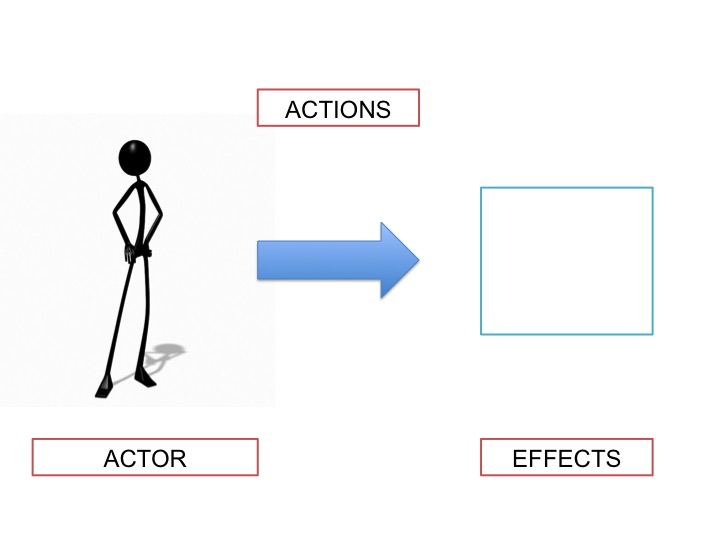
\includegraphics{Slide1.jpg}

\end{figure}

The first two theories we have discussed are action orientated. Each
agrees that the morality of an action in no way depends on the character
of the person it. On these views, being a good person is irrelevant to
the morality of your action. Virtue ethics is a radically different
view:

\begin{description}
\itemsep1pt\parskip0pt\parsep0pt
\item[Virtue Ethics:]
An action is permissible only if a virtuous person would perform it. An
action is impermissible only if a virtuous person would never perform
it.
\end{description}

Virtue Ethics traces its roots to the Ancient Greeks. Recall from the
introduction to this course that, for Socrates, the most important goal
in this life is to live a good life, to be a perfect a person. This, we
recall, was a dominant view among the Greeks. They cared about living
the best possible life, emulating their heroes, being recorded in the
annals of history, etc. Moral deliberation for the Greeks focused less
on what actions to perform and more on what kind of person to become.
This is a very different approach to ethics. It places constraints on
what kind of personality to develop. As such, the view can be more
demanding than the other two considered. It may take extensive therapy,
physical and mental training, as well extensive education to become a
good person.

Personalities are comprised of clusters of character traits. Virtue
Ethicists claim that a good person is one who has the best character
traits, which they call \textbf{virtues}. A bad person, on the other
hand, has the worse character traits, which are called \textbf{vices}.
According to the Virtue Ethicists, we must develop the virtues and stamp
out the vices. I'll first focus generally on character traits and
explain their relation to action. I'll then discuss how the Virtue
Ethicist selects some traits as virtues, others as vices.

\subsection{Character Traits}\label{character-traits}

Character traits are multi track dispositions to think, feel, and act in
certain ways. There are many such traits. Let us consider honesty as an
illustration.

What does it mean to call someone `honest'? On the one hand, it says
something about the way we expect the person \textbf{to act} in a
variety of different scenarios. If we were to offer an honest person a
chance to cheat on an exam, they will, of course, decline. If we ask an
honest person whether they studied for their exam, they will tell the
truth. If an honest person sees someone dropping a large sum of money,
we expect them to return it and not keep it.

By calling a person honest, we also are saying something how we expect
that person \textbf{to feel}. That is, there are a variety of emotions
that we expect an honest person to experience in certain scenarios. If
they watch a movie in which a person wins by deceit, they will feel
anger. They will feel sadness when watching an honest character fail in
their endeavors. We also can imagine that an honest person would feel
disgust if they were to witness cheating, pride if they saw their child
tell a difficult truth, guilt if they slipped and told a lie.

We also expect honest people \textbf{to think} in certain ways. An
honest person will think that, say, spying is not an admirable career;
they certainly will not be drawn to a life where they constantly must
lie. They may also have reservations about marketing and politics, but
hold in high regard investigative journalism.

Notice that being honest involves much more than merely acting honestly.
The idea here is that one has a trait, a disposition, from which honest
actions, emotions, and thoughts will flow. Just acting honest will never
make you honest. But being an honest person will lead you to act
honestly.

\subsection{Virtues and Vices}\label{virtues-and-vices}

Virtue Ethicists claim that some traits are virtues, some are vices.
What would make a trait one or the other? Perhaps the best known answer
comes from Aristotle, a student of Plato. Aristotle, born 384, was
Macedonian but moved to Athens to study with Plato. He ultimately
established his own school, the Lyceum, and is one of the most
influential, if not the most influential, philosopher of all time.

According to Aristotle, the traits which are virtues are those that
allow us to flourish as a human being. Some lives go well. Some lives go
poorly. Whatever enables a life to go well we should pursue. Whatever
prevents a life going well we should avoid. Obviously, then, we need to
try determine what it is for a life to go well, that is, what it is for
a person to flourish as a human being.

Aristotle's first move is to claim that x flourishes by realizing its
function. Consider a knife. A knife's job is to cut. A knife
\emph{flourishes} if it cuts well. It fails to flourish if it cuts
poorly. What characteristic must a knife have to cut well? Obviously,
sharpness. A blunt knife doesn't cut well. A sharp knife does. According
to Aristotle, then, sharpness is the virtue of a knife. It is what
allows the knife to perform its function well, i.e., it it is what
allows the knife to flourish.

Just as cutting is the activity characteristic of knives, Aristotle
thinks human flourishing consists in our characteristic activity, the
activity that humans and nothing else can engage in. According to
Aristotle, that activity is reasoning. Only we seem capable of
deliberating on what kind of life to live and how to figure out how to
live that life. Since virtues are what allow a thing to perform its
function well, a human's virtue will be what it allows humans to reason
well.

There is much to be said about what allows a human to reason well.
Aristotle offers a rich moral psychology that distinguishes, on the one
hand, those features a person must have if they are to follow the
dictates of their reason, and, on the other hand, those virtues that
will allow a person deliberate well.

For our purposes, we can ignore the complexities and focus on the kernel
of the view by way of illustration. If, say, we intend to pursue the
best career for ourselves, we will need to do two different things.
First, we'll need to form a judgement about the correct career, a
judgement that arises from deliberating on relevant things and not from
prejudices, odd desires, etc. If we are to act on that judgement, our
motives and desires better be in accord with that judgement. If, for
instance, you rationally decide that a music career is the one for you,
your desires and motivation better be in agreement with that decision,
e.g., you must be able to practice several hours a day, you must be
undistracted by pleasures, obstacles, and alternatives that will arise
as you practice.

The virtues, according to Aristotle, will be those character traits that
that allow us reason well and those that ensure we are able to obey the
dictates of our reasons. Our moral obligation, then, consists in
promoting and preserving these traits while constantly guarding against
anything which undermines them.

\end{document}
